\documentclass{article}
\usepackage{fontspec}
\pagestyle{empty}
\usepackage{geometry}
\geometry{paperwidth=100mm, paperheight=100mm, left=2mm, top=0mm, right=2mm, bottom=0mm}
\parindent=0pt
\usepackage{color}
\usepackage{xcolor}
\usepackage{tikz}

\begin{document}
\centering
\vspace*{\fill} \vspace*{-5ex}

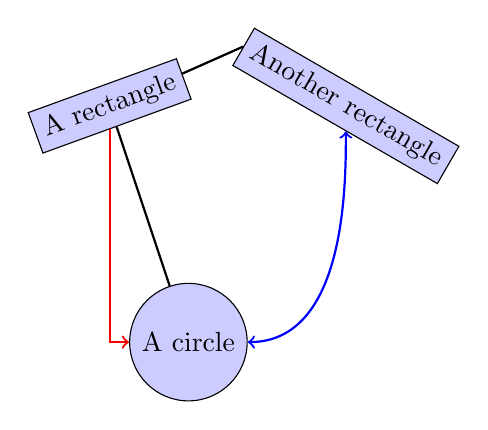
\begin{tikzpicture}[fill=blue!20]
\path (3,-1) node(b) [circle,draw,fill] {A circle}
(2,2) node(c) [rectangle,rotate=20,draw,fill] {A rectangle}
(5,2) node(d) [rectangle,rotate=-30,draw,fill] {Another rectangle};
\draw[thick] (b) -- (c) -- (d.west);
\draw[thick,red,->] (c) |- (b);
\draw[thick,blue,<->] (b) .. controls +(right:2cm) and +(down:1cm) .. (d);
\end{tikzpicture}

\vspace*{\fill} 
\end{document}